\documentclass[]{article}

\usepackage[a4paper, total={6in, 8in}]{geometry}

\usepackage[brazil]{babel}
\usepackage[utf8]{inputenc}

\usepackage{amsmath}
\usepackage{amsfonts}
\usepackage{amsthm}
\usepackage{listings}
\usepackage{hyperref}
\usepackage{graphics}
\usepackage{tikz}

\renewcommand{\baselinestretch}{1.4}
\setlength{\parindent}{2em}
\setlength{\parskip}{1em}

\begin{document}

\begin{center}
  \Large\textbf{Entrega 1} - \Large\textit{Daniel Brito}
\end{center}

\begin{center}
  \Large\textbf{Capítulo 1}
\end{center}

\noindent \textbf{5) Let $G$ be a graph of order 3 or more. Prove that $G$ is connected iff $G$ contains two distinct vertices $u$ and $v$ such that $G-u$ and $G-v$ are connected.}

IDA) Seja $G$ um grafo conexo. Como $G$ é conexo, logo, possui uma árvore geradora. Sabemos que uma árvore geradora é um subgrafo que contém todos os vértices de $G$, que é conexo e acíclico. Assuma que $p$ é um caminho maximal da árvore geradora de $G$, e que os vértices $u$ e $v$ são os extremos de $p$. Com isso, sabemos que as extremidades de $p$ possuem grau 1, pois, uma vez que o grau de um extremos é maior que 1, a maximalidade garante que o outro vizinho da folha além do seu antecessor teria que ser um vértice que pertence ao caminho, o que é um absurdo, visto que uma árvore geradora não possui ciclos. Portanto, como $u$ e $v$ possuem grau 1, podemos removê-las sem que isto impacte no restante do caminho de $p$, o qual ainda possui caminhos ligando os vértices remanescentes.

VOLTA) Seja $G-u$ um grafo conexo. Pela definição de conectividade, temos que existe um caminho que liga quaisquer par de vértices do grafo $G-u$. Incluindo um vértice $u$ ao grafo $G$, podemos afirmar que $u$ terá, pelo menos, um vizinho $w$. Além disso, como $G-u$ é conexo, temos que $w$ possui um caminho para qualquer outro vértice. Assim, com a aresta $uw$, $u$ consegue ter um caminho para qualquer outro vértice, uma vez que seu vizinho $w$ também possui.

\newpage

\noindent \textbf{24) Draw all of the (non-isomorphic) graphs of order 5.}

\begin{figure}[h]
	\begin{center}
		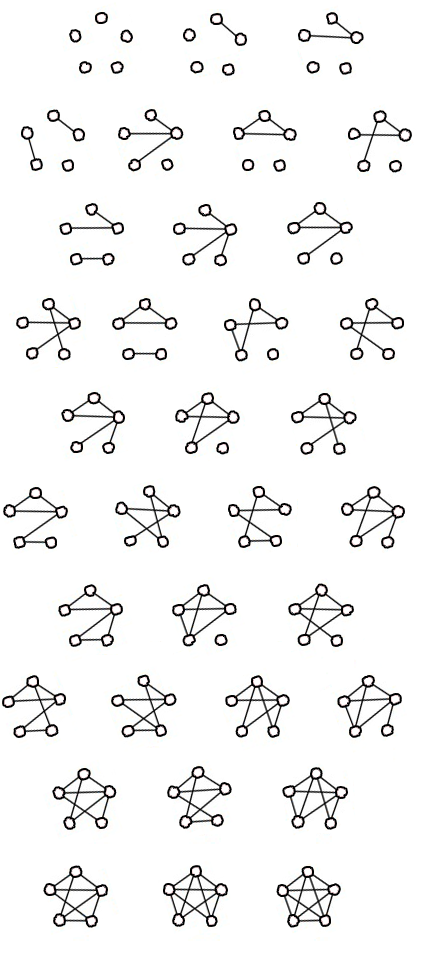
\includegraphics[scale=1.75]{image/graph.png}
	\end{center}
\end{figure}

\newpage

\noindent \textbf{12) For vertices $u$ and $v$ in a connected graph $G$, let $d(u, v)$ be the shortest length of a $u-v$ path in G. Prove that $d$ satisfies the triangle inequality.} 

Devemos mostrar que, dados os vértices $u, v, w \in G$, então, $d(u, w) \leq d(u, v) + d(v, w)$. Tal demonstração pode ser feita por contradição. Assim, assuma que $d(u, v) + d(v, w) < d(u, w)$. Pela definição, $d(u, v)$ é o tamanho do menor caminho de $u$ para $v$, e $d(v, w)$ é o tamanho do menor caminho de $v$ para $w$. Contudo, $d(u, w)$ é o tamanho do menor caminho de $u$ para $w$, logo, $d(u, v) + d(v, w)$ não pode ser menor que $d(u, w)$. Absurdo. Portanto, podemos concluir que $d$ satisfaz a desigualdade triangular.

\newpage

\noindent \textbf{19) Let $G$ be a graph of order $n$. Prove that if $deg(u) + deg(v) \geq n-1$ for every two nonadjacent vertices $u$ and $v$ of $G$, then $G$ is connected.}

Assuma que $u$ e $v$ não possuam um vizinho em comum, ou seja, $N(u) \cup N(v) = \emptyset$, onde $N(x)$ representa o conjunto de vizinhos de $x$. Assim, temos que $|N(u) \cup N(v)| = deg(u) + deg(v)$. Como $u$ e $v$ não possuem vizinhos em comum, então, $deg(u) \leq n-2 - deg(v)$, logo, $deg(u) + deg(v) < n-1$. Absurdo. Portanto, $u$ e $v$ devem possuir um vizinho em comum.

\newpage

\noindent \textbf{26) Prove that if $G$ is a disconnected graph then $\overline{G}$ is connected.}

Sabemos que $G$ é desconexo, então, existe um componente conexo $C$ tal que $V(C)$ contém, pelo menos, um vértice $v$, e existe, pelo menos, um vértice $w$ que está em $V(G)$, mas não está em $V(C)$. Precisamos mostrar que $\overline{G}$ é conexo. Assim, considere dois vértices quaisquer $x, y \in V(\overline{G}) = V(G)$, e também os seguintes casos:

\begin{itemize}
    \item Caso 1: $x, y$ estão ambos $V(C)$. Como $x$ e $w$ não estão no mesmo componente de $G$, $xw \notin E(G)$, logo, $xw \in E(\overline{G})$. Analogamente, $yw \in E(\overline{G})$. Assim, temos um caminho $x \rightarrow w \rightarrow y$ entre $x$ e $y$. 
    
    \item Caso 2: $x, y$ não estão em $V(C)$. Como $x$ e $y$ não estão no mesmo componente em $G$, $xv \notin E(G)$, logo, $xv \in (\overline{G})$. Analogamente, $yv \in E(\overline{G})$. Assim, temos um caminho $x \rightarrow v \rightarrow y$ entre $x$ e $y$.
    
    \item Caso 3: $x \in V(C)$ e $y \notin V(C)$. Com base nos casos anteriores, existe uma aresta entre $y$ e $v$. Além disso, $v$ e $x$ são conexos (Caso 1). Portanto, pela propriedade transitiva, temos que $y$ está conectado com $x$.
    
    \item Caso 4: $x \notin V(C)$ e $y \in V(C)$. Similar ao Caso 3, mas utilizando $w$ ao invés de $v$.
\end{itemize}

\newpage

\noindent \textbf{8) Prove that if $G$ is a nontrivial graph of order $n$ and size $m > \left( \begin{array}{c} n-1 \\ 2 \end{array} \right)$, then $G$ is connected.}

Podemos mostrar que todo par de vértices não-adjacentes possui um vizinho em comum. Baseado nesta ideia, para qualquer par de vértices $u, v$, temos que $uv \in E(G)$ ou existe um $x \in V(G)$ que é um vizinho comum de $u, v$. Assim, temos que $u \rightarrow x \rightarrow v$ é um caminho. Isto estabelece que todo par $u, v$ é conexo.

Considere qualquer par de vértices não-adjacentes. Seja $G'$ o subgrafo obtido a partir da remoção de $u$ e $v$ de $V(G)$, e todos as arestas incidentes em $u$ e $v$ de $E(G)$. Como $u$ e $v$ são não-adjacentes, temos: $m = |E(G)| = deg(u) + deg(v) + |E(G')| > \frac{(n-2)(n-3)}{2}$.Com isso, temos que $E(G') \leq \frac{(n-2)(n-3)}{2}$, uma vez que $G'$ possui $n-2$ vértices. Assim, $deg(u) + deg(v) > \frac{(n-1)(n-2)}{2} - \frac{(n-2)(n-3)}{2} = n-2$. Portanto, eles devem ter um vizinho comum entre os $n-2$ vértices remanescentes de $G'$.

\newpage

\noindent \textbf{22) Let $G$ and $H$ be isomorphic graphs. Prove the following.}

\noindent \textbf{(c) The graph $G$ is bipartie iff $H$ is bipartite.}

Seja $f: V(G) \rightarrow V(H)$ a bijeção que estabelece o isomorfismo.

$G$ é bipartido se, e somente se, H é bipartido. Como acima, basta que $G$ bipartido $\rightarrow$ $H$ é bipartido pela propriedade de simetria do isomorfismo. 

Seja $V(G) = V_1 \cup V_2$ uma partição em $G$. Seja $W_1 = \{f(x): x \in V_1\}$ e $W_2 = \{f(y): y \in V_2\}$. Verificamos que $V(H) = W_1 \cup W_2$ e $W_1 \cap W_2 = \emptyset$. Para qualquer vértice $a \in V(H)$, $f^{-1}(a)$ está em $V_1$ ou $V_2$. No primeiro caso, $a = f(f^{-1}(a)) \in W_2$, e no segundo caso, está em $W_2$. Então, $V(H) = W_1 \cup W_2$. Suponha que $W_1 \cap W_2 \neq \emptyset$, e seja $a \in W_1 \cap W_2$. Assim, $f^{-1}(a) \in V_1 \cap V_2$ contradiz o biparticionamento de $V(G)$. Agora, considere qualquer aresta $xy \in E(H)$. Isto implica que $f^{-1}(x) f^{-1}(y) \in E(G)$ seja a definição de isomorfismo. Portanto, $f^{-1}(x)$ e $f^{-1}(y)$ estão em diferentes lados em $G$. Podemos assumir que $f^{-1}(x) \in V_1$ e $f^{-1}(y) \in V_2$ (o caso reverso também tem um argumento semelhante). Por fim, pela definição $f(f^{-1}(x)) \in W_1$ e $f(f^{-1}(y)) = y \in W_2$, temos que os endpoints estão em lados diferentes de $H$.

\noindent \textbf{(d) The graph $G$ is connected iff $H$ is connected.}

Seja $f: V(G) \rightarrow V(H)$ a bijeção que estabelece o isomorfismo.

Como acima, basta que $G$ conexo $\rightarrow H$ é conexo pela propriedade de simetria do isomorfismo.

$G$ é conexo se, e somente se, H é conexo. Como acima, basta que $G$ conexo $\rightarrow$ $H$ é conexo pela propriedade de simetria do isomorfismo.

Considere quaisquer dois vértices $x, y \in V(G)$. Seja $u = f^{-1}(x) \in V(G)$ e $v = f^{-1}(y) \in V(G)$. Uma vez que $G$ é conexo, existe um caminho de $u$ até $v$: $ua_1a_2...a_kv$, onde $a_1, ..., a_k$ são os vértices intermediários do caminho. Então, $xf(a_1)f(a_2)...f(a_k)y$ é um caminho em $H$, logo, para quaisquer vértices consecutivos nesta sequência, temos que $f^{-1}$ mapeia para uma aresta no caminho em $G$.

\newpage

\noindent \textbf{11) Let $G$ be the graph with $\delta(G) = \delta$. Prove each of the following.}

\noindent \textbf{(a) The graph G contains a path of length $\delta$.}

Para $\delta=0$, a declaração é trivial, pois para qualquer vértice $v \in V$, a sequência $v$ forma um caminho de tamanho 0.

Assuma que $\delta \geq 1$. Seja $n$ o tamanho maximal de um caminho em $G$, e seja $v_1, v_2, ..., v_{n+1}$ tal caminho de tamanho $n$. Para provar (a), nós temos que mostrar que $n \geq \delta$.

Neste caso, podemos recorrer à uma demonstração por contradição, com $n < \delta$. Seja $S = N(v_{n+i} \ \{v_i | 1 \leq i \leq n\}$. Temos que $|S| \geq \delta(G)-n \geq \delta-n \geq 1$, ou seja, $S \neq \emptyset$. Tomemos um elemento $u \in S$. Então, a sequência $v_1, v_2, ..., v_{n+1}, u$ forma um caminho de tamanho $n+1$. Absurdo, pois assumimos que $n$ é tamanho maximal de um caminho em $G$.

\noindent \textbf{(b) If $\delta \geq 2$, prove that $G$ contains a cycle of length at least $\delta + 1$}.

Se $\delta(G)=1$, então $G$ não precisa ter ciclos.

Agora, assuma que $\delta \geq 2$. Como na demonstração anterior, seja $n$ o tamanho maximal de uma caminho em $G$, e seja $v_1, v_2, ..., v_{n+1}$ tal caminho de tamanho $n$. A partir de (a), temos que $n \geq \delta$. Assim, considere $S = N(v_{n+1} \ \{v_i | n-\delta+2 \leq i \leq n\}$.

Claramente, $|S| \leq \delta-(\delta-1)=1$, ou seja, $S \neq \emptyset$. Tomemos um elemento $u \in S$. Então, o trajeto $v_1, v_2, ..., v_{n+1}, u$ não pode ser um caminho, pois seu tamanho é $n+1 > n$. Isto significa que $u = v_m$, para algum $m \in [1, n-\delta+1]$, e então $v_m, v_{m+1}, ..., v_{n+1}$ é um caminho de tamanho $n+1-m+1 = n+2-m \geq n+2-(n-\delta+1)=\delta+1$.

\newpage

\noindent \textbf{21) Prove Theorem 1.8: If two graphs $G$ and $H$ are isomorphic, then (a) they have the same order and (b) the same size, and (c) the degrees of the vertices of $G$ are the same as the degrees of the vertices of $H$.
}

(a) Para que $G$ e $H$ sejam estruturalmente idênticos, deve haver uma bijeção dos vértices de $G$ para os vértices de $H$, em uma relação de 1 para 1, de tal forma que os conjuntos finitos tenham o mesmo tamanho. Com isso, resolvemos a questão da ordem, que é o número de vértices e o mesmo número de arestas.

Sejam $G$ e $H$ dois grafos isomórficos. Então, existe um isomorfismo $f: V(G) \rightarrow V(H)$ de $V(G)$ para $V(H)$. Seja sua inversa $f^{-1}: V(H) \rightarrow V(G)$ definida como sendo: $f^{-1}(v_2) = v_1 \iff f(v_1) = v_2$.

Sejam $u_2, v_2 \in V(H)$, tal que $f^{-1}(u_2) = u_1$ e $f^{-1}(v_2) = v_1$. Assim, $f(u_1) = (u_2)$ e $f(v_1) = v_2$. Então, $u_2$ e $v_2$ são adjacentes se, e somente se, $f(u_1)$ e $f(v_1)$ são adjacentes. Porque $G$ é isomórfico a $H$, $f(u_1)$ e $f(v_1)$ são adjacentes se, e somente se, $u_1 = f^{-1}(u_2)$ e $v_1 = f^{-1}(v_2)$ são adjacentes. Logo, $u_2$ e $v_2$ são adjacentes se, e somente se, $u_1 = f^{-1}(u_2)$ e $v_1 = f^{-1}(v_2)$ são adjacentes.

Portanto, $H$ também é isomórfico a $G$. Com isso, percebemos também que o isomorfismo preserva a simetria.

(c) Seja $f: V(G) \rightarrow V(H)$ a bijeção que estabelece o isomorfismo. Seja $u \in V(G)$ um vértice arbitrário de $G$, tal que $f(u) = v \in V(H)$. Seja $deg_G(u) = n$. Assim, precisamos mostrar que $deg_H(v) = n$.

Como $deg_G(u) = n$, existe $u_1, u_2, ..., u_n \in V(G)$ que são adjacentes a $u$. Qualquer outro vértice de $G$ não é adjacente a $u$.

Seja $f(u_i) = v_i$ para $1, 2, ..., n$. Uma vez que $f$ define um isomorfismo, cada um dos vértices $v_1, v_2, ..., v_n \in V(H)$ são adjacentes a $v$. De maneira análoga, qualquer outro vértice de $H$ não é adjacente a $v$.

Então, temos que $deg_H(v) = n$, o que se aplica para todos os vértices $u \in V(G)$.

\newpage

\begin{center}
  \Large\textbf{Capítulo 3}
\end{center}

\textbf{5) Prove that an Eulerian graph $G$ has even size iff $G$ has an even number of vertices $v$ such that $deg(v) \equiv 2 (mod \, 4)$}.

Seja o grafo $G$, com $m$ representando o número de arestas de $G$. Se $G$ é euleriano, então todos os nós têm grau par. Assim, seja $2a_i$ o grau do nó $i$. Com base no teorema de Teoria dos Grafos, temos que $m = \sum a_i$. Mas $a_i$ é par se, e somente se, o grau do nó $i$ é um múltiplo de 4, enquanto que é ímpar se, e somente se, o grau é $deg(i) = 2(mod \, 4)$. Então, a paridade de $m$ é decidida pela paridade de nós com $deg(i) \equiv 2(mod \, 4)$. Mais precisamente, $m$ tem a mesma paridade dos nós com $deg(i) \equiv 2(mod \, 4)$.

\newpage

\textbf{4) Prove or disprove: There exists a strong digraph with an Eulerian trail.}

\begin{figure}[h]
	\begin{center}
		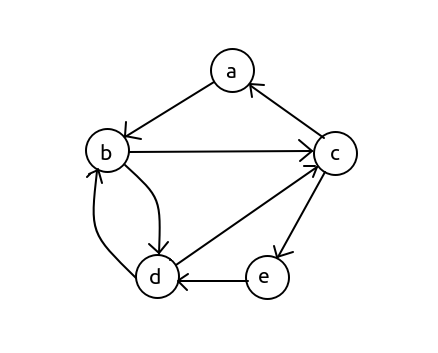
\includegraphics[scale=1]{image/prove.png}
	\end{center}
\end{figure}

% \hrulefill

% \textbf{NOTES:}

% \textbf{Strongly connected:} We say that a digraph $D$ is strongly connected if for every $u, v \in V (D)$ there is a directed walk from $u$ to $v$.

% \textbf{Eulerian trail:} A closed directed walk in a digraph $D$ is called Eulerian if it uses every edge exactly once. We say that $D$ is Eulerian if it has such a walk.

\newpage

\noindent \textbf{8)(a) Find an Eulerian circuit in the de Brujin digraph $B(2, 4)$ shown in Figure 3.6.}

\begin{figure}[h]
	\begin{center}
		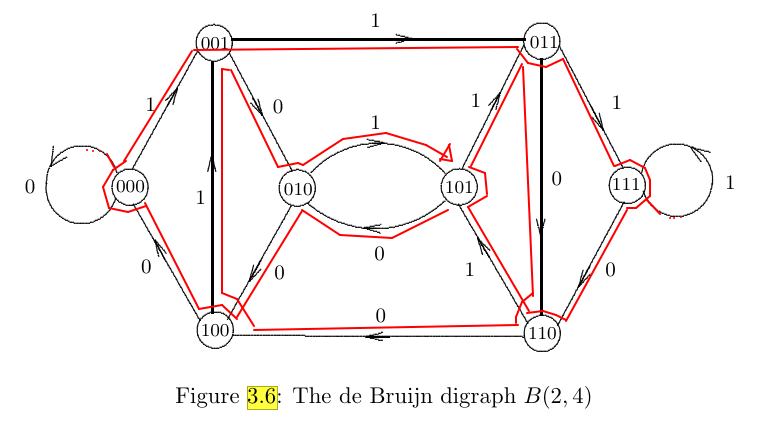
\includegraphics[scale=0.75]{image/brujin.png}
	\end{center}
\end{figure}

\noindent \textbf{(b) Use the information in (a) to construct the corresponding de Brujin sequence.}

Assuma que o caminho euleriano passa pelos vértices: 000, 000, 001, 011, 111, 111, 110, 101, 011, 110, 100, 001, 010, 101, 010, 100, 000. Assim, temos a seguinte sequência: 0000111101100101.

\noindent \textbf{(c) Locate the 4-words 1010, 0101, 1001, and 0110 in the de Brujin sequence in (b).}

\begin{itemize}
    \item 1010: ...0\}000111101100\{101...
    \item 0101: 000011110110\{0101\}
    \item 1001: 0000111101\{1001\}01
    \item 0110: 00001111\{0110\}0101
\end{itemize}

\newpage

\noindent \textbf{11) Prove that if $T$ is a tree of order at least 4 that is not a star, then $\overline{T}$ contains a Hamiltonian path.}

Vamos provar tal afirmação por meio de uma indução sobre a ordem $n$ de $T$. Para $n=4$, o caminho $P_4$ de ordem 4 é a única árvore de ordem 4, que não é uma estrela. Como $\overline{T} = T$, o resultado se mantém para $n=4$. Assuma que para toda árvore de ordem $k-1 \geq 4$, que não é uma estrela, seu complemento possui um caminho hamiltoniano.

Seja $T$ uma árvore de ordem $k$ que não é uma estrela. Então, $T$ possui um endpoint $v$, tal que $T-v$ não é uma estrela. Pela hipótese de indução, $\overline{T-v}$ possui um caminho hamiltoniano, dado por $v_1, v_2, ..., v_{k-1}$. Como $v$ é um end-point de $T$, isto significa que $v$ é adjacente a, no máximo, um de $v_1$ e $v_{k-1}$. Podemos assumir, sem perda de generalidade, que $v_1$ e $v$ não são adjacentes em $T$. Então, $v$ e $v_1$ são adjacentes em $\overline{T}$, e $v, v_1, v_2, ..., v_{k-1}$ é um caminho hamiltoniano em $\overline{T}$.

\newpage

\noindent \textbf{19) Prove that no bipartite graph of order 3 or more is Hamiltonian-connected.}

É suficiente mostrar que nenhum grafo bipartido completo é hamiltoniano conectado, pois qualquer grafo bipartido pode ser obtido a partir de um grafo completo por meio da remoção de arestas. E a remoção de arestas não pode tornar um grafo hamiltoniano conectado.

Assim, seja $G$ um grafo bipartido completo formado pelas partes $X$ e $Y$. 

Se $|X| = |Y|$, tome $u, v \in X$. Nenhum caminho hamiltoniano pode começar em $u$ e terminar em $v$, uma vez que qualquer caminho hamiltoniano partindo de $X$ deve terminar em $Y$.

Se $|X| < |Y|$, tome $u \in Y$ e $u \in X$. Nenhum caminho hamiltoniano pode começar em $u$ e terminar em $v$, uma vez que qualquer caminho hamiltoniano partindo de $Y$ deve terminar em $Y$. Para $|X| > |Y|$, temos uma situação análoga.

\newpage

\noindent \textbf{20) Give an example of a Hamiltonian graph $G$ and a path of order 2 in $G$, that cannot be extended to a Hamiltonian cycle of $G$.}

\begin{figure}[h]
	\begin{center}
		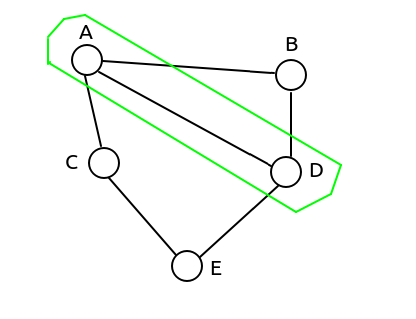
\includegraphics[scale=1]{image/path.png}
	\end{center}
\end{figure}

\newpage

\noindent \textbf{18) Prove that every Hamiltonian-connected graph of order 4 is 3-connected.}

Assuma que $G$ não é $3\mbox{-}connected$. Então, $G$ possui um corte de tamanho 2, digamos $\{x, y\}$. Suponha que este corte separa os vértices $a$ e $b$. Uma vez que $G$ é $4\mbox{-}ordered$ hamiltoniano, existe um ciclo em $G$ que possui os vértices $a, x, y, b$ nesta sequência. Agora, percorrendo de $a$ até $b$ neste ciclo, utilizando um caminho que evita $x$ e $y$, encontramos um caminho $a, b$ em $G-\{x, y\}$. Absurdo.

\end{document}